\documentclass[border=2pt]{standalone}
\usepackage{diagrams}
\usetikzlibrary{patterns,angles,quotes,arrows.meta,math,calc}
\usepackage{amsmath}
\tikzset{
  edge/.style={line width=1pt},
  vlbl/.style={font=\normalsize},
  elbl/.style={font=\small},
  dotnode/.style={circle, fill=black, inner sep=2pt},
}
\begin{document}
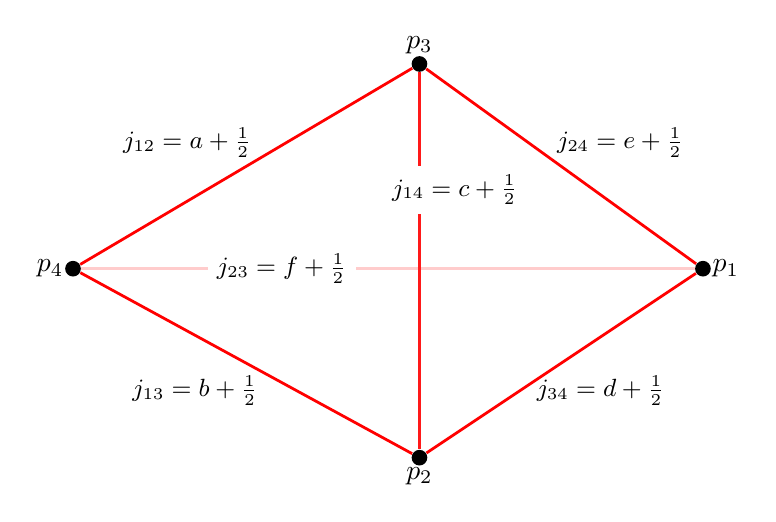
\begin{tikzpicture}[scale=1.0]
  \node[dotnode] (p3) at (0.4, 2.6) {};   % top
  \node[dotnode] (p2) at (0.4,-2.4) {};   % bottom
  \node[dotnode] (p4) at (-4, 0) {};      % left
  \node[dotnode] (p1) at ( 4, 0) {};      % right

  % six tetrahedron edges
  \draw[edge,color=red] (p4)--(p3) (p3)--(p1) (p4)--(p2) (p2)--(p1); % outer rhombus
  \draw[edge,color=red!20] (p4)--(p1);           % horizontal diagonal  j23
  \draw[edge,color=red!90] (p3)--(p2);           % vertical diagonal    j14

  % vertices
  \node[vlbl,above]      at (p3) {$p_3$};
  \node[vlbl,left]       at (p4) {$p_4$};
  \node[vlbl,right]      at (p1) {$p_1$};
  \node[vlbl,below]      at (p2) {$p_2$};

  % edge labels
  \node[elbl] at (-2.55, 1.6) {$j_{12}=a+\tfrac12$};
  \node[elbl] at ( 2.95, 1.60) {$j_{24}=e+\tfrac12$};
  \node[elbl] at (-2.45,-1.55) {$j_{13}=b+\tfrac12$};
  \node[elbl] at ( 2.7,-1.55) {$j_{34}=d+\tfrac12$};
  \node[elbl,fill=white] at (-1.35, 0) {$j_{23}=f+\tfrac12$};
  \node[elbl,fill=white] at ( 0.85, 1.00) {$j_{14}=c+\tfrac12$};
\end{tikzpicture}
\end{document}